% Indicate the main file. Must go at the beginning of the file.
% !TEX root = ../main.tex

%%%%%%%%%%%%%%%%%%%%%%%%%%%%%%%%%%%%%%%%%%%%%%%%%%%%%%%%%%%%%%%%%%%%%%%%%%%%%%%%
% 03_results
%%%%%%%%%%%%%%%%%%%%%%%%%%%%%%%%%%%%%%%%%%%%%%%%%%%%%%%%%%%%%%%%%%%%%%%%%%%%%%%%

\section{Results}
\label{results}

\subsection{Detection}
One of the main goals of the initial detection through the dataset was to identify which images were suitable for the training routine.
The selection of images and the discarded ones are shown in \autoref{tab:data_availability_after_md}; the data is divided into four categories.
The effect of the selection is displayed for detection thresholds of \(0.25\) and \(0.5\), with the latter being the one finally applied.
On the image level, the most affected category is \textit{soricidae}, with \(23\%\) of the images being discarded, followed by \textit{mustela\_erminea} with \(20\%\).
The other categories, \textit{apodemus\_sp} and \textit{cricetidae}, were only affected by \(7\%\) and \(8\%\), respectively.
On the sequence level, the situation is very different, with only the \textit{mustela\_erminea} category being seriously affected, with \(23\%\) of the sequences being discarded.
For the other categories, only around \(1\%\) of the sequences were discarded.
Some visual examinations of the results of the \ac{MD} were performed to gain a better understanding of the outcomes --- some of these insights are presented in the following, focusing on the \textit{mustela\_erminea} category.
Some of the highest-confidence detections for this category are shown in \autoref{fig:detection_mustela_best}; all the images display a properly detected animal.
The inspection of images with no detection within a threshold of \(0.25\) is shown in \autoref{fig:detection_special_nodetect}; this is a hand-picked selection of images that were interesting for the analysis.
Most of the images with no detection were actually empty or showed only the tip of the animal's tail, as seen in examples (c)--(g).
Some showed forms of obstruction, such as examples (a) and (b), with the dragged-in tube in (b) being a common one.
There were also several images with an animal clearly visible but no detection, such as in examples (h)--(l).
This occurred far more often for individuals with white fur than for those with brown fur --- this observation is based on visual inspection and has not been statistically evaluated.

% table
\begin{table}[ht]
\centering
\caption{Data loss dew to \acs{MD} output for confidence thresholds of \(0.25\) and \(0.5\) by category for the image and the sequence level.}
\label{tab:data_availability_after_md}
\begin{tabular}{l r r r r}
\toprule
 & \texttt{apodemus\_sp} & \texttt{cricetidae} & \texttt{mustela\_erminea} & \texttt{soricidae} \\
\midrule
\midrule
\textbf{Image Level} & & & & \\
Total available & 279,492 & 156,350 & 16,465 & 16,645 \\
\midrule
Threshold of \(0.25\): & & & & \\
Lost & 16,609 & 9,248 & 2,914 & 3,529 \\
Percentage lost & 6\% & 6\% & 18\% & 21\% \\
Available & 262,883 & 147,102 & 13,551 & 13,116 \\
\midrule
Threshold of \(0.5\): & & & & \\
Lost & 19,417 & 11,948 & 3,290 & 3,865 \\
Percentage lost & 7\% & 8\% & 20\% & 23\% \\
Available & 260,075 & 144,402 & 13,175 & 12,780 \\
\midrule
\textbf{Sequence Level} & & & & \\
Total available & 13,669 & 5,329 & 1,035 & 2,107 \\
\midrule
Threshold of \(0.25\): & & & & \\
Lost & 51 & 40 & 211 & 7 \\
Percentage lost & 0\% & 1\% & 20\% & 0\% \\
Available & 13,618 & 5,289 & 824 & 2,100 \\
\midrule
Threshold of \(0.5\): & & & & \\
Lost & 56 & 46 & 239 & 13 \\
Percentage lost & 0\% & 1\% & 23\% & 1\% \\
Available & 13,613 & 5,283 & 796 & 2,094 \\
\bottomrule
\end{tabular}
\end{table}

\begin{figure}[]
\centering
\includegraphics[width=\textwidth]{figures/mustela_best.pdf}
\caption{Highest confidence value detections for the category \textit{mustela\_erminaea} category.}
\label{fig:detection_mustela_best}
\end{figure}

\begin{figure}[]
\centering
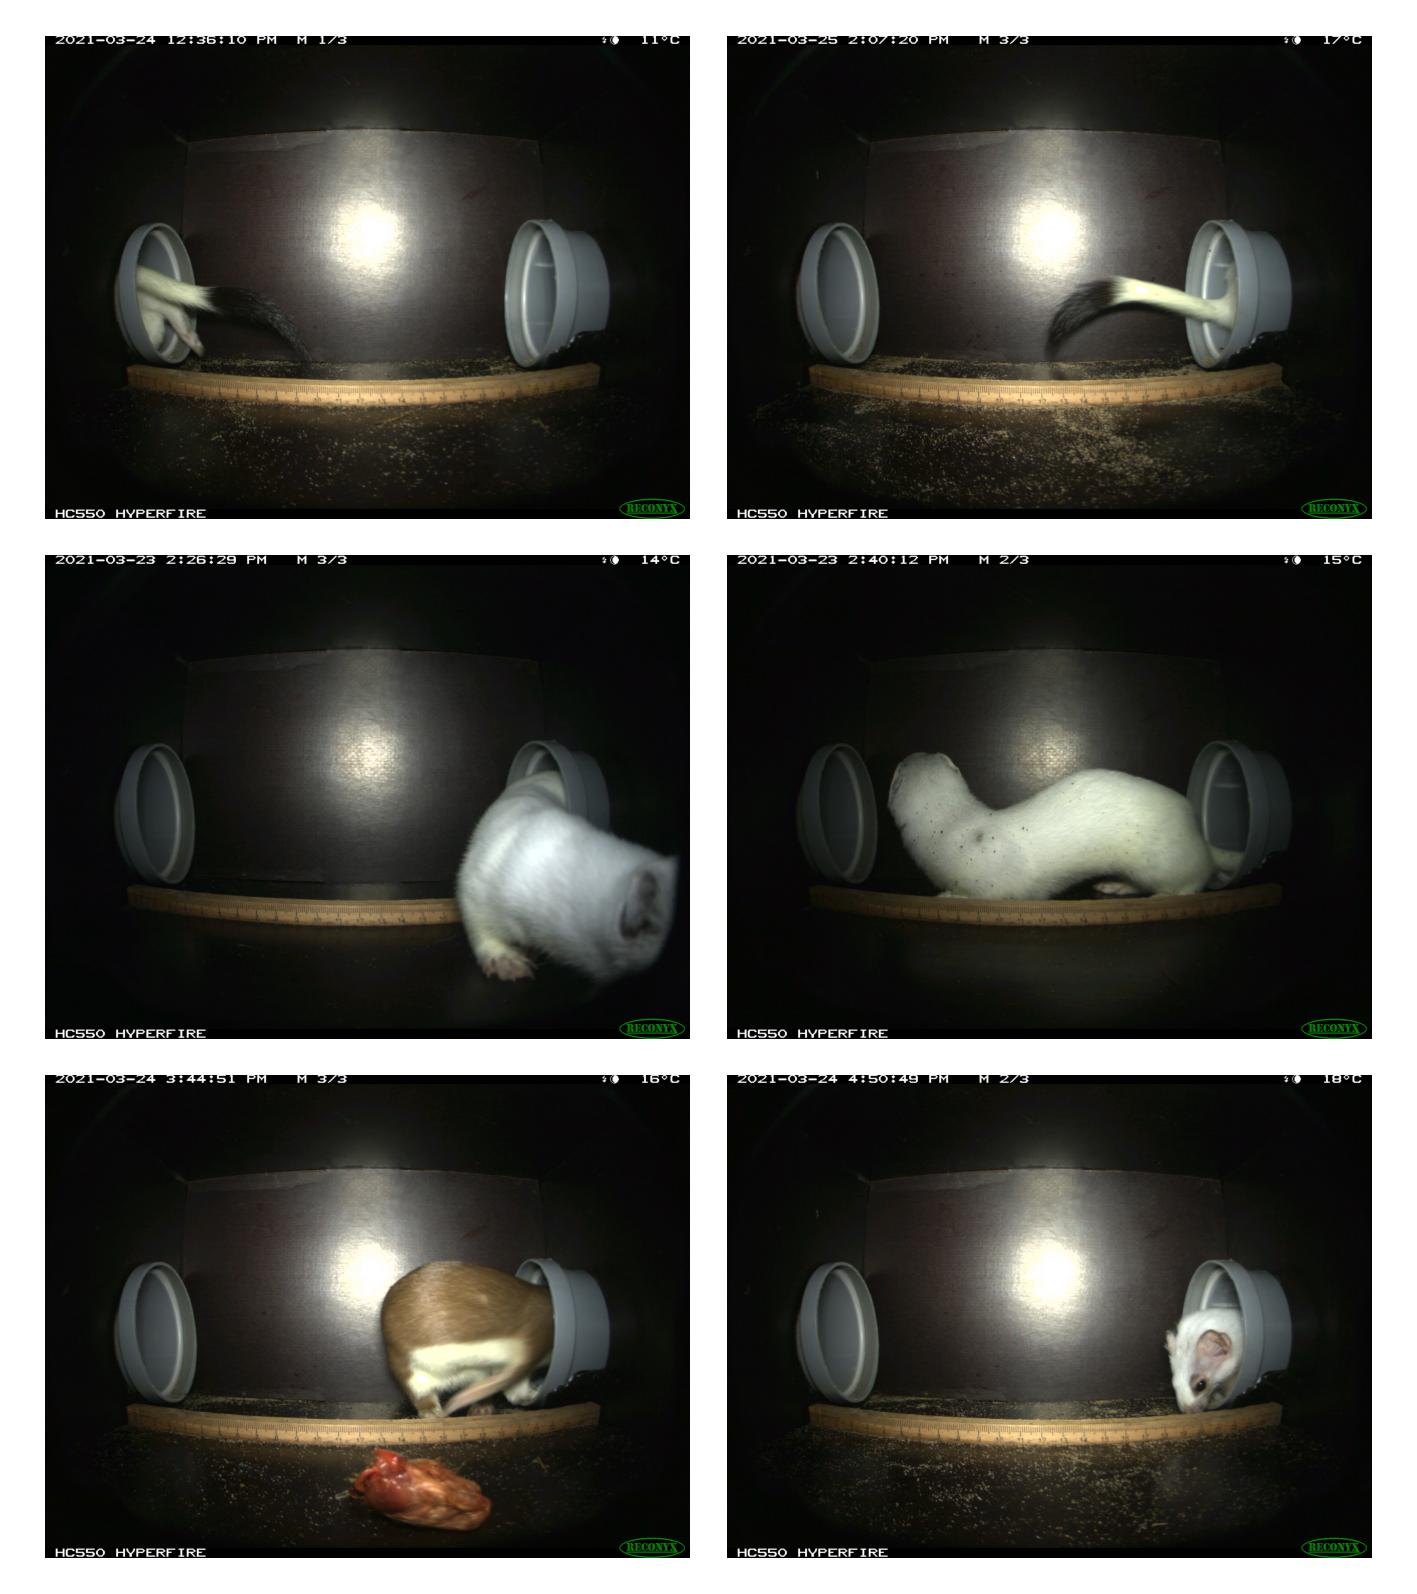
\includegraphics[width=\textwidth]{figures/mustela_special_nodetect.pdf}
\caption{Hand-picked selection of interesting images of the \textit{mustela\_erminea} category with no detection within a threshold of \(0.25\).}
\label{fig:detection_special_nodetect}
\end{figure}

\subsection{Classification Performance}
All classification models performed well on their respective test sets.
The \ac{BA} scores for each model are presented in \autoref{tab:bal_acc_by_model}.
Generally, smaller models achieved slightly higher scores than larger ones, although these differences remained within one standard deviation.
In particular, the pretrained EfficientNet-B0 reached the highest \ac{BA} of \(0.992\pm0.004\).
Applying sequence-level classification to the image-level predictions improved \ac{BA} for every model, but only by \(0.001\) to \(0.005\), which again falls within a single standard deviation.

Pretrained models consistently outperformed those trained from scratch, as shown in \autoref{fig:bal_acc_img} and \autoref{tab:bal_acc_by_model}.
EfficientNet-B0 with pretraining performed uniformly well across all folds, with only one outlier, while the non-pretrained version scored slightly lower on average and showed greater variability.
In contrast, DenseNet-169 showed less of a gap between pretrained and non-pretrained variants, with the pretrained version performing slightly better but also showing increased spread across folds.
ResNet-50 values were more dispersed for both variants, yet the pretrained model still held a clear advantage.
Finally, ViT-B/16 displayed the largest benefit from pretraining, alongside the greatest fold-to-fold variability in both its pretrained and non-pretrained versions.

% table
\begin{table}[H]
\centering
\caption{Balanced accuracy of all models -- shown as mean ± standard deviation.}
\label{tab:bal_acc_by_model}
\begin{tabular}{l c r c c}
\toprule
Model & Pretrained & Params (M) & Image BA-Score & Sequence BA-Score \\
\midrule
efficientnet\_b0 & Yes & 4 & 0.9921 ± 0.004 & 0.9947 ± 0.002 \\
densenet169 & Yes & 12 & 0.9904 ± 0.004 & 0.9939 ± 0.002 \\
resnet50 & Yes & 23 & 0.9899 ± 0.004 & 0.9934 ± 0.002 \\
vit\_b\_16 & Yes & 85 & 0.9885 ± 0.005 & 0.9933 ± 0.002 \\
\midrule
efficientnet\_b0 & No & 4 & 0.9856 ± 0.005 & 0.9898 ± 0.003 \\
densenet169 & No & 12 & 0.9863 ± 0.006 & 0.9899 ± 0.002 \\
resnet50 & No & 23 & 0.9850 ± 0.004 & 0.9888 ± 0.003 \\
vit\_b\_16 & No & 85 & 0.9767 ± 0.006 & 0.9856 ± 0.004 \\
\bottomrule
\end{tabular}
\end{table}\todo{highlight the best model}

\begin{figure}[ht]
\centering
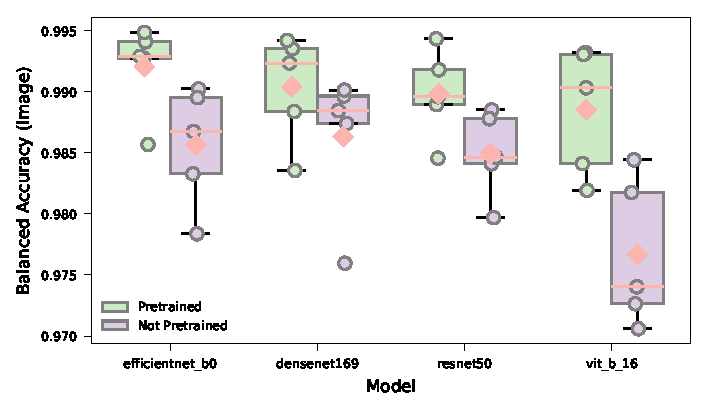
\includegraphics{figures/bal_acc_img.pdf}
\caption{\acs{BA} of each model on the image-level across folds, shown separately for pretrained and non-pretrained variants. Individual fold results are plotted as points; the mean \acs{BA} is marked by a diamond; and the median is indicated by a horizontal line.}
\label{fig:bal_acc_img}
\end{figure}

\subsection{Best Performing Model Architecture}
The model architecture with the best performance measured by \ac{BA} was EfficientNet-B0 with pretraining.
In \autoref{fig:training_metrics_best_model}, the validation loss and \ac{BA} across training epochs for all cross-validation folds are shown.
For all folds, the best version, defined by the lowest validation loss, occurred within the first 3 epochs, while the \ac{BA} kept increasing.

Its performance per category is shown in \autoref{tab:precision_recall_fscore_support}.
The class it performed best on was \textit{mustela\_erminea}, with a value of \(0.999\) for all metrics --- this happens to be one of the classes with relatively few samples available.
It performed the worst on the other underrepresented class, \textit{soricidae}, with a precision of \(0.971\), recall of \(0.979\), and F1-score of \(0.975\).
For the other, more represented classes, the model achieved very high scores above \(0.99\) for all metrics.

The normalized \ac{CM} for the best model is shown in \autoref{fig:conf_matrix_best}.
It shows that there were essentially no false positives for the class \textit{mustela\_erminea}, while it was rarely confused with other classes.
The most frequent misclassification occurred with \textit{soricidae} being falsely classified as \textit{apodemus\_sp}, with a value of \(0.0184\).
All other classes had a false positive rate of less than \(0.006\).

The Spearman correlation between the detection confidence and the classification confidence is:\todo{change this to corellation coefficient}

\begin{tabular}{l l l}
For correct predictions: & $\rho = 0.092$ & $p < 10^{-300}$ \\
For incorrect predictions: & $\rho = 0.276$ & $p = 3.0 \times 10^{-39}$ \\
\end{tabular}

This shows that there is a very weak positive correlation between detection confidence and classification confidence for correctly classified images, and a weak positive correlation for misclassified images.
The $p$-values are far below the significance threshold of \( \alpha = 0.05 \), indicating that both correlations are statistically significant.

\begin{figure}[ht]
\centering
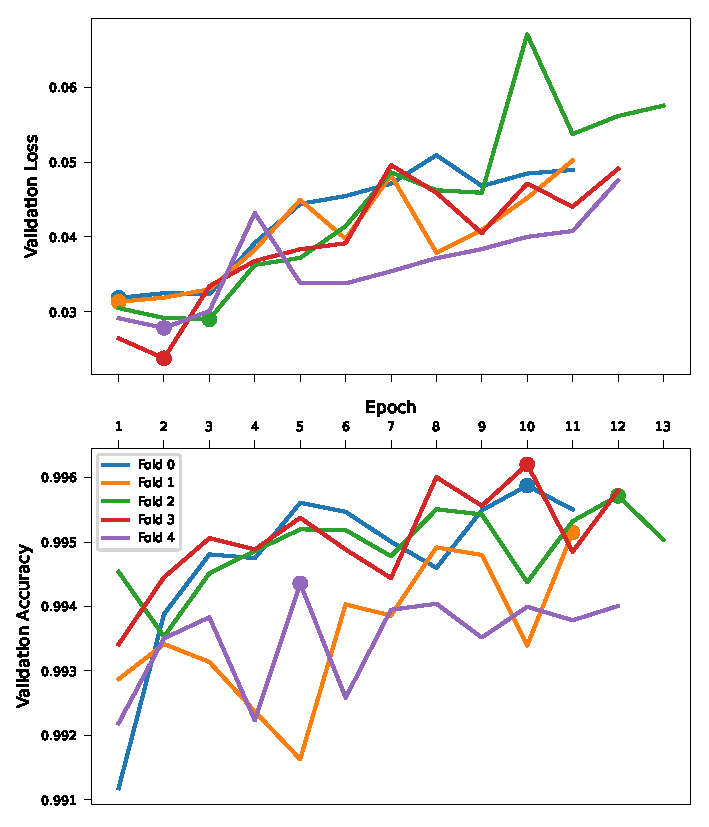
\includegraphics{figures/training_metrics_best_model.pdf}
\caption{Validation Loss and \acs{BA} across training epochs for the best-performing model, shown for all cross-validation folds. In the Validation Loss subfigure, the lowest value per fold is marked with a dot to indicate the best epoch. In the \acs{BA} subfigure, the highest value per fold is similarly marked.}
\label{fig:training_metrics_best_model}
\end{figure}\todo{why is this val loss so much lower as in other eval?}    

% table
\begin{table}[H]
\caption{Precision, recall and F1-score for the best model.}
\label{tab:precision_recall_fscore_support}
\begin{tabular}{l r r r r}
\toprule
Class & Precision & Recall & F1-Score & Support \\
\midrule
apodemus\_sp & 0.996 & 0.997 & 0.996 & 260075 \\
mustela\_erminea & 0.999 & 0.999 & 0.999 & 13175 \\
cricetidae & 0.995 & 0.993 & 0.994 & 144402 \\
soricidae & 0.971 & 0.979 & 0.975 & 12780 \\
\bottomrule
\end{tabular}
\end{table}


\begin{figure}[ht]
\centering
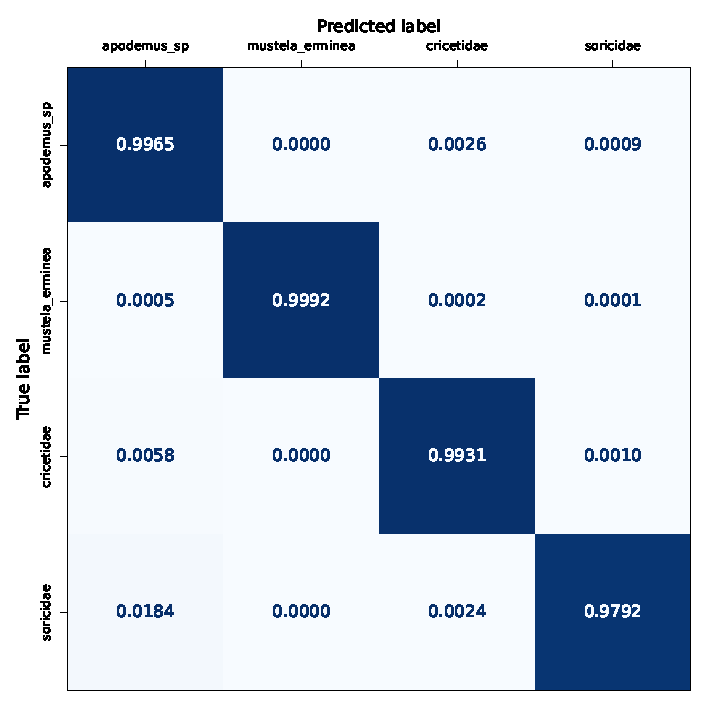
\includegraphics{figures/conf_matrix_best.pdf}
\caption{Normalized \acs{CM} for the best-performing model.}
\label{fig:conf_matrix_best}
\end{figure}